\documentclass{beamer}
\mode<presentation>

\usepackage{enumerate}

\title{Young Tableaux: una implementazione}
\author[Campagni]{Candidato: Alessandro Campagni \medskip \\Relatore:
  Marco Maggesi}
\date{}

\usetheme{CambridgeUS}

\begin{document}

\begin{frame}
\titlepage
\end{frame}

%% \frame{\tableofcontents}

\section{Preliminari}
\subsection{Diagrammi di Young}

\begin{frame}
\frametitle{Diagramma di Young}
\begin{columns}[T]
\column{5cm}
\includegraphics[width=0.6\textwidth]{images/YoungDiagram.pdf}
\column{5cm}
$11=4+3+2+1+1$
\end{columns}
\end{frame}

\begin{frame}
\frametitle{Diagramma coniugato}
\begin{columns}[T]
\column{5cm}

\includegraphics[height=0.6\textwidth]{images/YoungDiagramTransposed.pdf}
\column{5cm}
$11=5+3+2+1$
\end{columns}
\end{frame}

\begin{frame}
\frametitle{Skew diagram}
\centering
\begin{columns}
\begin{column}<1->{3.3cm}
\includegraphics[width=0.7\textwidth]{images/skew_diag_1.pdf}\\
$\lambda=(5,3,2)$
\end{column}
\begin{column}<2->{3.3cm}
\includegraphics[width=0.7\textwidth]{images/skew_diag_2.pdf}\\
$\mu=(2,1)$
\end{column}
\begin{column}<3->{3.3cm}
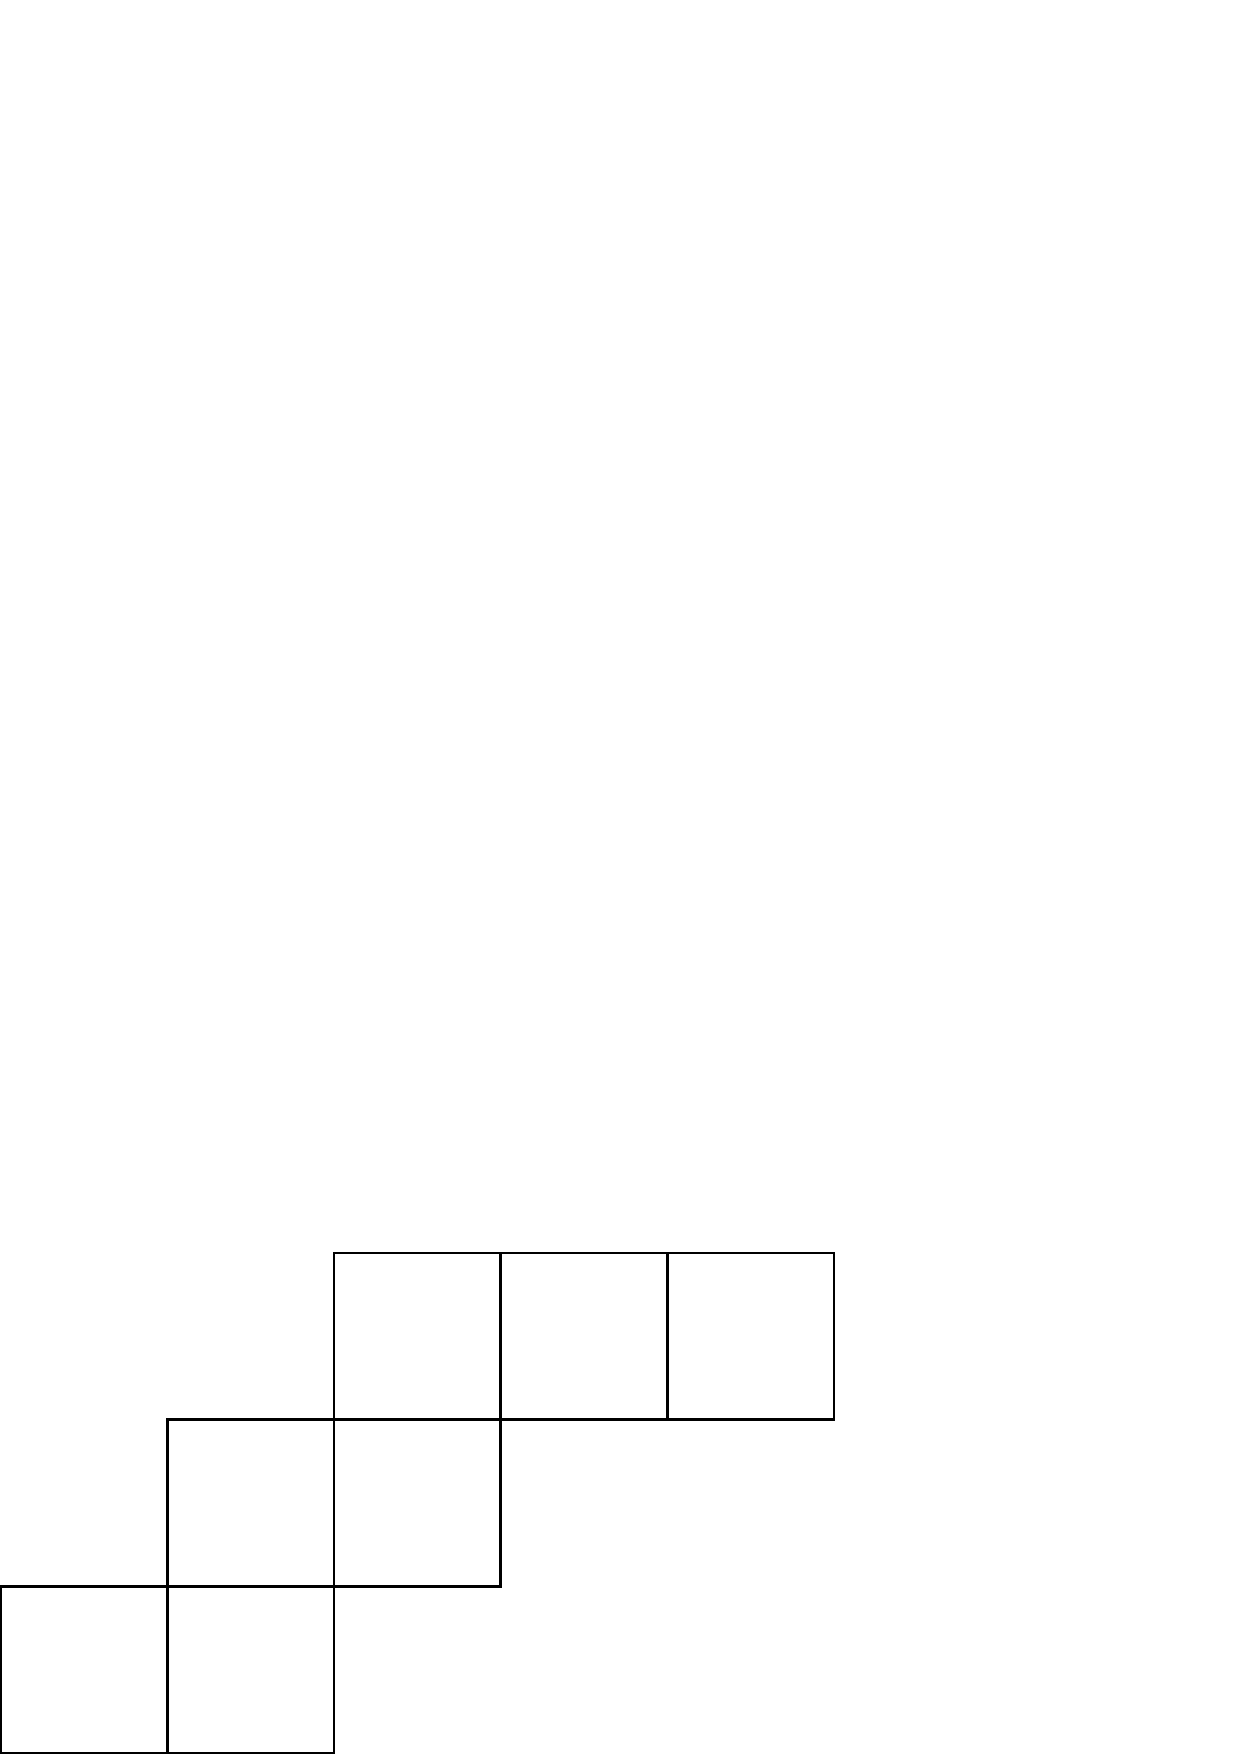
\includegraphics[width=0.7\textwidth]{images/skew_diag_3.pdf}\\
$\lambda / \mu$
\end{column}
\end{columns}
\end{frame}

\subsection{Young tableaux}

\begin{frame}
\frametitle{Young tableau}
\begin{columns}
\column{5cm}
\includegraphics<1->[width=0.7\textwidth]{images/tableau.pdf}
\column{5cm}
\begin{enumerate}[(i)]
\item<2-> $T^i_j \leq T^i_{j+1}$
\item<3-> $T^i_j < T^{i+1}_j$
\end{enumerate}
\end{columns}
\end{frame}

\begin{frame}
\frametitle{Row bumping}
\centering
\begin{columns}[t]
\begin{column}{3.3cm}
\includegraphics<1->[height=0.7\textwidth]{images/bump_1.pdf}\\
\includegraphics<4->[height=0.6\textwidth]{images/bump_4.pdf}
\end{column}
\begin{column}{3.3cm}
\includegraphics<2->[height=0.6\textwidth]{images/bump_2.pdf}\\
\includegraphics<5->[height=0.6\textwidth]{images/bump_5.pdf}
\end{column}
\begin{column}{3.3cm}
\includegraphics<3->[height=0.6\textwidth]{images/bump_3.pdf}\\
\includegraphics<6->[height=0.6\textwidth]{images/bump_6.pdf}
\end{column}
\end{columns}
\end{frame}

\begin{frame}
\frametitle{Prodotto di tableaux}
\centering
\begin{columns}[t]
\begin{column}{5cm}
\includegraphics<1->[width=0.7\textwidth]{images/prod_1.pdf}\\
\includegraphics<3->[width=0.6\textwidth]{images/prod_3.pdf}
\end{column}
\begin{column}{5cm}
\includegraphics<2->[width=0.7\textwidth]{images/prod_2.pdf}\\
\includegraphics<4->[width=0.5\textwidth]{images/prod_4.pdf}
\end{column}
\end{columns}
\end{frame}

%% \subsection{Skew tableau}

\section{Polinomi di Schur}

\section{Littlewood-Richardson}

\end{document}
